%\part{Referencial Teórico}

\chapter[Referencial Teórico]{Referencial Teórico}
Nesta seção do artigo serão explicados conceitos importantes para realização do projeto, especificação de alguns materiais e a motivação para a escolha dos mesmos.  
	\section{Sensores Inerciais em Humanos}
% VER QUALIFY GILMAR	
%	Os avan¸cos dos sensores MEMS foram fortemente impulsionados e alavancados com informa
%	¸c˜oes e tecnologias de comunica¸c˜ao, com integra¸c˜ao de circuitos de baixa pot^encia,
%	comunica¸c˜ao sem fio m´odulos e redes de sensores sem fio, permitindo o design de compacto,
%	alto desempenho, baixo consumo de energia e solu¸c˜oes de baixo custo para uma
%	ampla gama de aplica¸c˜oes (MAGNO et al., 2013) (DAVIS, 2010).
%	Neste contexto, o dom´ınio da sa´ude e do bem-estar representa um dos setores
%	mais atraentes com um alto potencial para contribuir com o crescimento do mercado e
%	o desenvolvimento do sensor MEMS tecnologia (KUMAR; JYOTHSNA, 2013). Sensores
%	port´ateis, descart´aveis e para cuidados de sa´ude, e tamb´em para detec¸c˜ao de atividades,
%	para o bem-estar em geral s˜ao usadas para monitorar, por exemplo, frequ^encia
%	card´ıaca, press˜ao sangu´ınea, respira¸c˜ao, bem como para realizar diagn´osticos espec´ıficos
%	de doen¸cas; eles tamb´em incluem sistemas para cuidar de um envelhecimento crescente
%	da popula¸c˜ao e pacientes cronicamente doentes.
%	O uso de Sensores para monitorar doen¸cas cr^onicas, como hipertens˜ao, obesidade,
%	diabetes, dist´urbios do sono e falhas no cora¸c˜ao, ´e o elemento-chave para manter a qualidade
%	de vida elevada (muitas vezes prevendo o evento) e tamb´em para reduzir o custo dos
%	cuidados de sa´ude gra¸cas a um monitoramento remoto. Al´em disso, a interven¸c˜ao precoce
%	´e vital para pacientes com risco de desenvolver doen¸cas cr^onicas (HUFF, 2014).
%	Nos ´ultimos anos, os Sistemas Micro-Electro-Mec^anicos Biom´edicos ou Biol´ogicos
%	(BioMEMS) t^em mostrado um enorme potencial para o campo biom´edico, tanto de um
%	ponto de pesquisa como industrial de Vis˜ao. Os dom´ınios de aplica¸c˜ao mais promissores
%	dizem respeito, diagn´ostico avan¸cado, terapia e tecido estrat´egias de engenharia. Na ´area
%	de an´alise e detec¸c˜ao biomol´eculas, o BioMEMS atualmente exerce um papel significativo,
%	fornecendo plataformas para detectar microrganismos, cadeias de DNA, mol´eculas, v´ırus
%	e c´elulas (FOLADORI et al., 2016).
%	Um n´umero significativo de estudos j´a foram realizados na avalia¸c˜ao da Doen¸ca
%	de Parkinson (PD), considerado um modelo de desordem para defici^encia motora (BATTISTA;
%	SCORZA; SCIUTO, 2012). Em geral, sensores de movimento, tais como como
%	aceler^ometros e girosc´opios, s˜ao usados em combina¸c˜ao com luz, geralmente flex´ıveis e
%	eletr^onicos confort´aveis que n˜ao interferem com movimento e atividades humanas normais.
%	Uma fundamental vantagem em compara¸c˜ao com os sistemas tradicionais de avalia
%	¸c˜ao cl´ınica ´e que esses sensores garantem uma avalia¸c˜ao mais objetiva, quantitativa e
%	20
%	confi´avel dos sintomas; eles tamb´em mostram significativa vantagens comparadas `as tecnologias
%	laboratoriais (por exemplo, captura de movimento optoeletr^onico - MOCAP),
%	pois permitem longas monitoramento de prazo em cen´arios da vida real (HOBERT et al.,
%	2014).
%	Na ci^encia do esporte os MEMS baseados em sensores surgiram recentemente como
%	um elemento-chave, bem como em v´arios dom´ınios da vida di´aria relacionadas com entretenimento
%	e lazer. Neste quadro, v´arias pesquisas t^em fortemente beneficiado de medidas
%	quantitativas ativadas por tecnologias de detec¸c˜ao diferentes, aplicadas a segmentos corporais,
%	ambientes ou ferramentas de trabalho, al´em de estarem “conquistando” v´arios tipos
%	de modalidades de esportes. Os dispositivos inteligentes est˜ao cada vez mais emergente
%	para monitorar as atividades em uma ampla gama de esportes, bem como para movimentos
%	e mapeamento dos atores de rastreamento em anima¸c˜ao para efeitos especiais em
%	filmes (JOHNSON, 2012).
	
	
	\section{MEMS}

		MEMS\footnote{Micro Electro Mechanical Systems - Sistema Micro-eletromecânicos}  é uma tecnologia de processamento usada para criar dispositivos integrados ou sistemas que combinam componentes mecânicos e elétricos. Eles são fabricado usando técnicas de processamento em lote de circuitos integrados e pode variar em tamanho entre alguns micrômetros para milímetros. Esses dispositivos (ou sistemas) têm a capacidade de detectar, controlar e atuar na escala micro e gerar efeitos em escala macro\cite{prime2002}. 

		O termo MEMS, é um acrônimo originado nos Estados Unidos, também é conhecido como Microsystems Technology (MST) na Europa e Micromachines no Japão. Independentemente da terminologia, o fator de define um dispositivo MEMS está na maneira como é feito. Enquanto os aparelhos eletrônicos são fabricados usando tecnologia IC de 'chip de computador', os componentes micromecânicos são fabricados por sofisticadas manipulações com silício e outros substratos usando processos de micro-usinagem. Processos como micro-usinagem a granel e de superfície, bem como micromaquinação de alta proporção (HARM \footnote{high-aspect-ratio micromachining}) remove seletivamente partes do silício ou adiciona camadas estruturais adicionais para formar os componentes mecânicos e eletromecânicos. Enquanto circuitos integrados são projetados para explorar as propriedades elétricas do silício, o MEMS aproveita as propriedades mecânicas do silício ou suas propriedades elétricas e mecânicas\cite{prime2002}.

		Na forma mais geral, os MEMS consistem em microestruturas mecânicas, microssensores, microatuadores e microeletrônica, todos integrados no mesmo chip de silício (Fig. \ref{esquematico_mems}). Microsensores detectam mudanças no ambiente do sistema medindo informações ou fenômenos mecânicos, térmicos, magnéticos, químicos ou eletromagnéticos. Microeletrônica processa essa informação e sinaliza aos microatuadores para reagirem e criarem alguma forma de mudanças no meio ambiente\cite{prime2002}.

		\begin{figure}[h]
			\centering
			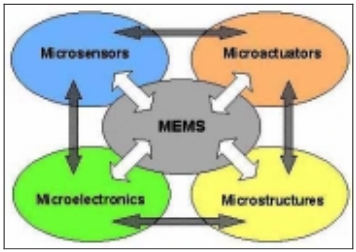
\includegraphics[keepaspectratio=true,scale=0.5
			]{figuras/esquematico_mems.png}
			\caption{Ilustração esquemática de componentes MEMS}
			Fonte: \cite{prime2002}
			\label{esquematico_mems}
		\end{figure}

		Os dispositivos MEMS são muito pequenos, seus componentes são geralmente microscópicos(Fig. \ref{escala_mems}). Alavancas, engrenagens, pistões, motores e até motores a vapor foram todos fabricados por MEMS. No entanto, MEMS não se refere apenas à miniaturização de componentes mecânicos ou à fabricação de coisas a partir do silício (na verdade, o termo MEMS é na verdade enganoso, já que muitos dispositivos micromachinados não são mecânicos em nenhum sentido). MEMS é uma tecnologia de fabricação; um paradigma para projetar e criar dispositivos e sistemas mecânicos complexos, bem como sua eletrônica integrada, utilizando técnicas de fabricação em lote\cite{prime2002}.

		\begin{figure}[h]
			\centering
			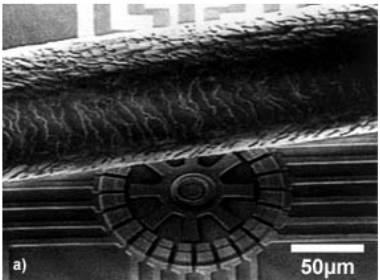
\includegraphics[keepaspectratio=true,scale=0.5
			]{figuras/escala_mems.png}
			\caption{Um motor MEMS ao lado de uma fio de cabelo humano.}
			Fonte: \cite{prime2002}
			\label{escala_mems}
		\end{figure}

	\section{IMU}

		A história do sensor IMU começou em 1930, quando foi usado para auxiliar a navegação de aeronaves e outros dispositivos de grande porte. Por causa de suas restrições principalmente em tamanho, custo e consumo de energia, o uso da IMU naquele momento era restrito a aplicações em dispositivos grandes e, portanto, impopular para equipamentos de tamanho menor e em grande escala de consumo. Porém, recentemente, o sensor IMU feito por MEMS, foi introduzido com uma característica muito atraente de baixo custo, com poder de processamento e baixo custo. A demanda aumentou muito e as áreas de aplicação também. Atualmente, muitos fabricantes estão competindo nos melhores projetos de IMU, como Invensense, Honeywell, STMicroelectronics, Microstrain e X-Sens\cite{ahmad2013}.
		
		Os sensores IMU podem ser capazes de medir diversas variáveis. Os mais comuns são feitos para medir 6 graus de liberdade. São 3 medidas de aceleração linear a partir de um acelerômetro e 3 medidas de aceleração angular feitas por um giroscópio (Fig.\ref{eixos_imu})\cite{santos2016}.
		 
		\begin{figure}[h]
			\centering
			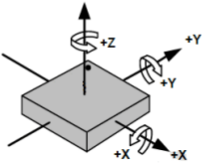
\includegraphics[keepaspectratio=true,scale=0.8]{figuras/Eixos_imu.png}
			\caption{Eixos de orientação.}
			Fonte adaptada de \cite{mpu6050}
			\label{eixos_imu}	
		\end{figure}


		A vantagem de usar este tipo de IMU é que não será interferido pelo campo magnético externo em torno do
		sensor quando é usado muito próximo de material ferromagnético. Por outro lado, dependendo do acelerômetro e do giroscópio, pode não ser suficiente para aumentar a precisão da medição devido ao ruído dos sensores e à questão do desvio do giroscópio. Os dados adquiridos pelo IMU são integrados como a mostrado na Figura \ref{integracao_imu} \cite{ahmad2013}.

		\begin{figure}[h]
			\centering
			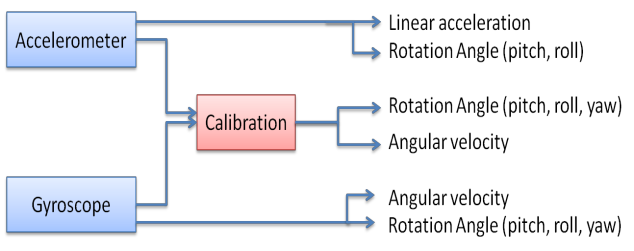
\includegraphics[keepaspectratio=true,scale=0.3
			]{figuras/integracao_imu.png}
			\caption{Sensor inercial baseado em 2 sensores}
			Fonte adaptada de \cite{ahmad2013}
			\label{integracao_imu}
			
		\end{figure}

		E com essas variáveis adquiridas um padrão de movimento pode ser traçado, e assim podem ser feitas análises sobre a movimentação humana. Assim, junto com a EMG\footnote{Eletromiografia}, o uso de sensores inercias tem sido mais solicitado na área de monitoramento de práticas esportivas\cite{howard2016}.
		
		Porém, a utilização de IMU's com equipamentos de comunicação sem fio, têm mostrado uma certa vantagem sobre o uso de sensores com EMG. Isso ocorre por conta de a integração entre acelerômetros, giroscópios e dispositivos de transmissão sem fio ser mais simplificada do que a aquisição de dados por eletromiógrafos sem fio\cite{howard2016}. 
		
		Os testes que foram feitos com uso de sensores inerciais, segundo  Howard,2016 , foram capazes de produzir dados relacionados com fadiga muscular, performance, postura e velocidade. O que possibilita melhores técnicas de treinamento e até mesmo prevenção de lesão pode ser realizada.

			\subsection{Acelerômetro}
			
				O que sensores de movimento são feitos para aferir uma taxa de variação de posição, ou seja o deslocamento que estiver ocorrendo. Assim, se a posição, $x(t)$, de um corpo varia ao longo tempo, então será obtida sua velocidade, $v(t)$,  derivando essa mudança de posição ao longo do tempo. E ao derivar a variação de velocidade ao longo do tempo será calculada a aceleração, $a(t)$, do corpo \cite{moyses2013}.
				\begin{equation}
				v(t) = \frac{dx(t)}{dt}
				\end{equation}
				
				\begin{equation}
				a(t) = \frac{dv(t)}{dt} = \frac{d^2v(t)}{dt^2} 
				\end{equation}
				
				Um acelerômetro é capaz de medir a aceleração, e a partir desse dado é possível obter também a velocidade e posição. Basta fazer a operação inversa a derivada\cite{moyses2013}.
				
				\begin{equation}
				v(t) = v(0) + \int_{0}^{1}(a(t)dt)
				\end{equation}
				\begin{equation}
				x(t) = x(0) + \int_{0}^{1}(v(t)dt)
				\end{equation}
				
				Acelerômetros podem ser utilizados em muitas áreas, como na  automotiva com air bags, na navegação,no monitoramento de máquinas, na saúde, jogos e outras. São diversos os processos físicos utilizados para desenvolver um sensor para
				medir aceleração. Em aplicações que envolvem voo, aviões e satélites,
				acelerômetros são baseados em propriedades de massas rotativas. Na industria,
				porém, o projeto mais comuns são feitos a partir da combinação da lei de Newton de
				aceleração de massa e a lei de Hooke de ação de mola \cite{carneiro2003}.
				
				O acelerômetro escolhido para esse trabalho funciona a partir do efeito de cristais piezoelétricos, que é o princípio no qual alguns cristais geram uma corrente elétrica como resposta a uma pressão mecânica. Então o sensor acelerômetro  funciona como na Figura \ref{acel} demonstra, como uma pequena caixa com uma esfera dentro, e as paredes são os cristais piezoelétricos.  Sempre que a caixa é alterada de posição a esfera é forçada a se mover em direção de uma das paredes devido a força da gravidade ou de qualquer outra força de aceleração em outro sentido que não a normal. Cada par de paredes paralelos correspondem a um eixo no espaço. Assim, a partir da corrente gerada em cada parede é possível determinar a direção do movimento acelerado e sua magnitude \cite{Sanjeev2018}.
				
				\begin{figure}[h]
					\centering
					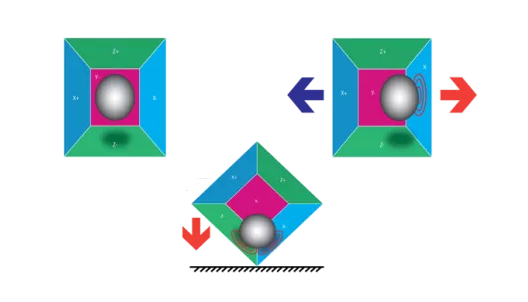
\includegraphics[keepaspectratio=true,scale=0.8
					]{figuras/acelerometro.PNG}
					\caption{Princípio de funcionamento do acelerômetro.}
					Fonte adaptada de \cite{Sanjeev2018}
					\label{acel}
				\end{figure}
	
		\subsection{Giroscópio}
			
			Os giroscópios também são sensores de movimento, porém eles não medem aceleração linear como os acelerômetros, eles disponibilizam ao usuário a velocidade angular de um objeto em torno de um eixo. Em geral, os giroscópios feitos com tecnologia MEMS utilizam do efeito Coriolis, no qual um objeto que se encontra em um movimento de rotação, imprime na massa um movimento ortogonal a direção de rotação. Os giroscópios têm um princípio muito mais complexo que os acelerômetros, este e um dos motivos fizeram eles demorarem mais a parecer como dispositivos MEMS \cite{almeida2014}.
			
			O giroscópio do tipo diapasão, modelo utilizado no trabalho, é constituído por duas massas paralelas que oscilam com a mesma amplitude, direção igual e sentidos opostos mostrado na Figura .
			
			\begin{figure}[h]
				\centering
				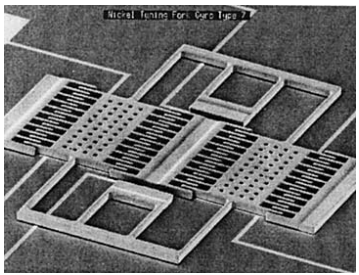
\includegraphics[keepaspectratio=true,scale=0.7
				]{figuras/diapasao.png}
				\caption{ Imagem de microscopia eletrônica por varredura de um giroscópio diapasão.}
				Fonte adaptada de \cite{forhan2010}
				\label{gyro}	
			\end{figure}
			
			Ao acontecer uma rotação, a força de Coriolis gera uma vibração ortogonal ao sentido do movimento de cada massa. A amplitude desse movimento pode ser medido de forma capacitiva. A utilização de dois giroscópios na mesma direção e em sentidos opostos aumenta a precisão da medição. Com a medida da força de Coriolis  $F_{c}$, a medida da massas paralelas $m$, se movendo a um determinada velocidade $v$, com relação a um referencial fixo que possua uma velocidade angular $ \omega $ é possível obter a aceleração de Coriolis $a_{c}$. \cite{forhan2010}.
			
			\begin{equation}
			F_{c} = 2mv\omega
			\end{equation}
			
			\begin{equation}
			a_{c} = 2v\omega
			\end{equation}
			
			Com aceleração de Coriolis que é obtido pelo sensor a unidade de processamento do sensor é capaz de calcular a velocidade angular em $\degree$/s. Com a velocidade angular em relação a cada eixo do espaço tridimensional sendo obtida, é possível encontrar posição angular do sensor e do objeto, ou corpo, em que ele estiver acoplado \cite{forhan2010}\cite{moyses2013}. 
			
			A unidade de medida padrão de velocidade angular  é rad/s. Então, com o intuito de converter o valor obtido para o padrão internacional:
			
			\begin{equation}
			1 \pi rad = 180\degree
			\end{equation}
			
			\begin{equation}
			1 \pi rad /s = 180\degree/s 
			\end{equation}
			
			\begin{equation}
			 \frac{\pi}{180} rad /s = (\frac{180}{180})\degree/s 
			\end{equation}
			
			\begin{equation}
			\frac{\pi}{180} rad /s = 1\degree/s 
			\end{equation}

%Os giroscópios são similares em operação aos acelerômetros; no entanto, eles são usados ​​para detectar a velocidade angular, geralmente com uma saída de graus por segundo. Essa funcionalidade os torna muito úteis em conjunto com acelerômetros para um sistema que requer rastreamento de movimento confiável.

\subsection{MPU6050}
	
	O MPU6050, é da séria MPU60X0, foi a primeira interface de movimento a integrar 6 eixos de leitura em um dispositivo único. Esse sensor de movimento, integra 3 eixos de um acelerômetro e 3 eixos de um gyroscópio e um DMP \footnote{\textit{Digital Motion Processor} - Processador Digital de Moviemento} tudo em um pequeno componente medindo 4x4x0.9mm. As suas principais qualidades são seu tamanho reduzido, o baixo consumo de energia, alta precisão e confiabilidade, alta tolerância a choques mecânicos, tem seu desempenho programável para aplicações específicas e ainda um baixo custo finaceiro. \cite{mpu6050}.
	
	O protocolo de comunicação utilizado pelo MPU6050 é o I2C\footnote{\textit{Inter-Integrated Circuit} - Circuito Inter-Integrado}. Que é um protocolo de barramento, e com os mesmos dois fios podem ser conectados vários dispositivos, um sendo o \textit{master} e os outros como \textit{slave}. Esta é uma característica boa para reduzir a quantidade de pinos necessários para conexão de mais dispositivos no microcontrolador.\cite{mpu6050}
	
	As aplicações, sugeridas pelo fabricante, para o MPU6050 são diversas, abaixo estão listadas algumas delas:
	\begin{itemize}
		\item Tecnologia \textit{ BlurFree\texttrademark }\footnote{Para estabilização de imagens e videos.}
		\item Controles para jogos baseados em movimento
		\item Sensores em roupas TouchAnywhere para aplicação na saúde e esportes
		\item Tecnologia \textit{ MotionCommand\texttrademark}\footnote{Para comandos de movimento curtos} 
		\item Em brinquedos
	\end{itemize}
	
	\begin{description}
		\item[Características do MPU6050] 
		\item \begin{itemize} 
			\item  O giroscópio, MEMS de 3 eixos do MPU6050, possui as seguintes características segundo \cite{mpu6050}:
			\begin{itemize}
				\item Saídas digitais com os valores de velocidade angular para os eixos X,Y e Z com escalas progrmáveis entre $ \pm250 $,$ \pm500 $,$ \pm1000 $ e $ \pm 2000$ $\degree$/seg
				\item Conversores ADCs\footnote{Analog Digital Converter - Conversor Analógico Digital} de 16 bits integrados permitem amostragem simultânea do giroscópio
				\item Corrente de operação: 3.6mA
				\item Bom desempenho com ruído de baixa frequência
				\item Filtro passa-baixa programável.
				\item Fator de escala de sensibilidade calibrado de fábrica.
			\end{itemize}
			\item O acelerômetro, MEMS de 3 eixos do MPU6050, possui as seguintes características segundo \cite{mpu6050}:\begin{itemize}
				\item Saídas digitais dos 3 eixos do acelerômetro com escalas programáveis entre $\pm2g$, $\pm4g$, $\pm8g$ e $\pm16g$. Sendo \textquoteleft$ g$\textquoteright \ uma constante que equivale a aceleração da gravidade\footnote{aproximadamente $9,81 m/s^2 $}
				\item Conversores ADCs de 16 bits integrados permitem amostragem simultânea do acelerômetro sem a necessidade de um multiplexador
				\item Orientação, detecção e sinalização
				
			\end{itemize}
		\end{itemize}
	\end{description}
	
	
	

\subsection{Arduino}

O Arduino é uma plataforma de desenvolvimento de código aberto que contém elementos de hardware e software especificamente adaptados à simplicidade de uso, permitindo uma rápida prototipagem de projetos. Placas Arduino têm grande potencial de desenvolvimento e uma ampla gama de recursos para uso em conjunto com sensores, transceptores de dados e atuadores, os quais são de grande interesse para este projeto \cite{smith2016}.

Uma das maiores vantagens do Arduino sobre outra plataformas de prototipagem com microcontroladores é a facilidade para utiliza-la, que permite que pessoas que não necessariamente são da área de tecnologia, possam aprender rapidamente o básico e criar seus próprios projetos. E existe um grande compartilhamento de projetos de forma livre utilizando essa plataforma. Isso é relevante para esse projeto em específico, pois ele está sendo desenvolvido para utilização de pesquisadores de diversas áreas do conhecimento. Os quais poderão aprender a adaptar o projeto para suas necessidades e demandas futuras \cite{arduino2011}.

Existem diversos modelos de placas Arduino no mercado, as mais utilizadas são Lilypad, Uno, Mini Pro, Mega e Nano. Cada uma dessas placas possuem suas particularidades em relação ao número de recursos, formato físico, memória e capacidade de processamento. Na Tabela \ref{tipos_arduino} estão listados alguns modelos e suas características \cite{smith2016}.


\begin{table}[h] \footnotesize
	\centering
	\caption{Tabela de comparação dos modelos de Arduino}
	\label{tipos_arduino}
	
	\begin{tabular}{lccccc}
		\toprule
		\textbf{Modelos} & \textbf{Lilypad} & 
		\textbf{Uno} & \textbf{Pro} & \textbf{Mega}  & \textbf{Nano} \\
		\midrule
		Microcontrolador & ATmega32u4 & ATmega328P & ATmega238 & ATmega2560 & ATmega328P \\
		Tensão de Operação & 3.3V & 5V & 3.3/5V & 5V & 5V \\
		Tensão de Entrada & 3.8-5V & 7-12V & 5-12V & 7-12V & 5-12V \\
		Pinos Digitais & 9 & 14 & 14 & 54 & 14 \\
		Entradas Analógicas & 4 & 6 & 6 & 16 & 8 \\
		Memória Flash & 32kB & 32kB & 32kB & 256kB & 32kB \\
		Velocidade do Clock & 8MHz & 16MHz & 8/16MHz & 16MHz & 16MHz \\
		Dimensões Físicas & 50mm$\oslash$ & 68.6 x 53.4mm & 52 x 53mm & 101.5x53.5mm &  18,5 x 43,2mm \\
		Custo Aproximado & R\$ 22,00 & R\$ 54,00 &  R\$ 50,00 & R\$ 80,00 & R\$ 24,00 \\
		\bottomrule
		Fonte adaptada: & \cite{smith2016}
	\end{tabular}
\end{table}

O  modelo escolhido para este projeto foi o Arduino Nano, mostrado na Figura \ref{arduino} , pois mesmo sendo apenas um protótipo, haverá a necessidade de que o tamanho do IMU seja reduzido para facilitar a fixação em diversas partes do corpo e o custo financeiro\footnote{Preços pesquisados em lojas de Brasília.} para desenvolvimento do protótipo foi levado em consideração.

\begin{figure}[h]
	\centering
	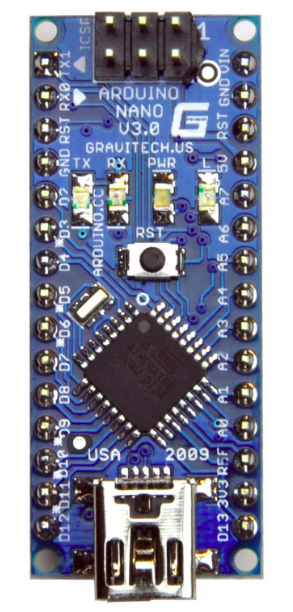
\includegraphics[keepaspectratio=true,scale=0.7
	]{figuras/arduino_nano.png}
	\caption{ Arduino Nano }
	Fonte adaptada de \cite{john2018}
	\label{arduino}	
\end{figure}


O Arduino Nano tem funcionalidades muito semelhantes às do Arduino Duemilanove, mas com um formato diferente. O Nano possui o microcontrolador ATmega328P embutido nele, o mesmo que o Arduino UNO. A principal diferença entre eles é que a placa UNO é apresentada em formato PDIP\footnote{Plastic Dual-In-line Package} com 30 pinos e Nano está disponível em PQFP\footnote{Plastic Quad Flat Pack} com 32 pinos. Os 2 pinos extras do Arduino Nano servem para as funcionalidades do ADC, enquanto o UNO possui 6 portas ADC, o Nano possui 8. A placa Nano não vem com um conector para fonte DC\footnote{Direct Current - Corrente Contínua} como outras placas Arduino, mas possui uma porta mini-USB. Esta porta é usada para programação, monitoramento serial e alimentação de energia, se necessário. A característica fascinante do Nano é que ele escolherá a fonte de energia mais forte com sua diferença de potencial, e o \textit{jumper} de seleção de fonte de energia é inválido\cite{john2018}.  

Para se comunicar com qualquer microcontrolador ou computador, é necessário usar uma linguagem de programação, no caso do Arduino, é necessário usar a linguagem C++\footnote{Com alguma modificações}, que é uma linguagem tradicional e já bastante conhecida. Porém essa linguagem ainda não é a que a máquina compreende, é uma linguagem de alto nível, e para a máquina compreende-la é necessário o uso de um compilador, que converte a linguagem de alto nível para a linguagem de máquina. Em geral, para compilar um programa é necessário a utilização de um IDE\footnote{Integrated Development Environment}, um aplicativo de computador que possui um compilador integrado. A plataforma do Arduino utiliza o Arduino IDE\cite{chavier2016}. 


\section{Python}

Python é uma linguagem de programação poderosa, mas fácil de usar, desenvolvida por Guido van Rossum, em 1991. Com o Python, você pode escrever rapidamente um pequeno projeto e também, por se adaptar bem, pode ser usado para aplicativos comerciais. Uma prova de como é um linguagem comercial é ela ser utilizada por empresas como Google, IBM, NASA, Xerox, Yahoo e outras grandes empresas \cite{dawson2010}.

O principal objetivo de qualquer linguagem de programação é fazer uma ponte entre o programador e a máquina. E as maioria das linguagens de programação tornam esse comunicação mais próxima da humana, mas o Python é tão direto que, segundo \cite{dawson2010}, é chamada de "programação na velocidade do pensamento", essa facilidade se traduz na alta produtividade de programadores profissionais. Os quais com ele conseguem fazer programas mais curtos e mais rápidos de escrever do que com outras linguagens de programação. 

Python é uma boa linguagem para aplicações científicas porque é fácil traduzir raciocínio em algoritmos através dela, é simples ler um código em Python e conseguir entender o raciocínio por trás dele, por ser uma linguagem com poucos caracteres especiais, poucas palavras chaves utilizadas apenas para compilar e ter uma sintaxe muito próxima da linguagem falada \cite{reitz2018}.

Além disso, é uma linguagem de propósito geral. Muitas vezes, é necessário lidar com tarefas laterais: buscar dados em um banco de dados remoto, ler uma página na internet, exibir graficamente os resultados, criar uma planilha, etc. Linguagens de cunho especificamente científico têm um sério problema aí, mas, uma vez que Python é utilizada em praticamente todos os tipos de tarefa, encontram-se módulos prontos para realizar essas tarefas que podem se tornar complicadas. Ou seja, é uma preocupação a menos para quem está desenvolvendo aplicações científicas \cite{downey2012}.
  





\chapter[Metodologia]{Metodologia}

Nesta seção será apresentado quais foram os materiais e métodos utilizados para implementação do projeto, tanto da parte de hardware(parte de física) quanto a parte de software. A principal metodologia utilizada foi baseada  em scrum, que é um método ágil iterativo incremental, onde o projeto foi divido em ciclos de 15 dias chamados de "\textit{sprints}". A cada \textit{sprint}, algumas atividades são retiradas do \textit{backlog}\footnote{Conjunto de requisitos que ainda não foram solucionados.}, colocadas no campo "\textit{do}"\footnote{Campo onde estão as atividades a serem realizadas durante a \textit{sprint}.}  e tem de ser resolvidas até a o início da próxima \textit{sprint}, onde as atividade realizadas serão avaliadas,  validadas ou não, se estiverem atendendo ao requisito são enviadas para o "\textit{done}"\footnote{Conjunto de atividades que já foram feitas e validadas}, se não estiverem atendendo as necessidades, elas voltam ao \textit{backlog} ou para o \textit{do}.

Os resquisitos do projeto, que compuseram o backlog e definiram os objetivos desse projeto foram relacionados com o auxílio dos pesquisadores do Laboratório de Informática e Saúde e alunos de mestrado da UnB.

\section{Projeto de Hardware}


 
	\subsection{Materiais Utilizados}
		\begin{itemize}
			
			\item sensor MPU6050;
			\item Arduino Nano V.3;
			\item Fios(\textit{jumpers};
			\item Cabo USB;
			\item Computador com Arduino IDE e Python instalados;
			\item Jupyter Notebook;
			\item Tiras de velcro;
			\item Cabo flat (8 fios);
			\item Protoboard.
			
		\end{itemize}	
	 
	\subsection{Métodos}
		
		Para realizar a comunicação do sensor MPU6050 com o Arduino foi feita a conexão conforme o esquemático mostrado na Figura \ref{conexoes} e a Tabela \ref{conexoes_arduino} , logo abaixo, onde os pinos Vcc e Gnd do MPU6050, responsáveis por ligar do sensor, foram conectados aos pinos 5V e Gnd do Arduino, o pino SDA\footnote{Pino de transferência de dados} foi conectado ao pino SDA do Arduino, que também é o pino de entrada analógica A4 e o pino SCL\footnote{Pino de sincronização do \textit{clock}} ao pino SCL do Arduino, que também é o pino de entrada analógica A5.  
		
		Para os primeiros testes foi utilizada um \textit{protoboard} para facilitar as conexões, pois ela permite que os componentes sejam conectado sem a necessidade de solda entre eles. Mas em um segundo momento para os teste de movimento serem realizados com maior acurácia, houve a necessidade de retirar os componentes da \textit{protoboard} e soldá-los em um placa furada de cobre, e isso faria o ruído devido a conexões instáveis fosse menor.
		\begin{table}[h] \footnotesize
			\centering
			\caption{Conexões entre Arduino e MPU6050}
			\label{conexoes_arduino}
			
			\begin{tabular}{cc}
				\toprule
				\textbf{Arduino} & \textbf{MPU6050} \\
				\midrule
				5V & VCC \\
				GND & GND \\
				A4 & SDA \\
				A5 & SCL \\
				\bottomrule
				Fonte: & autoria própria
			\end{tabular}
		\end{table}
		
		\begin{figure}[h]
			\centering
			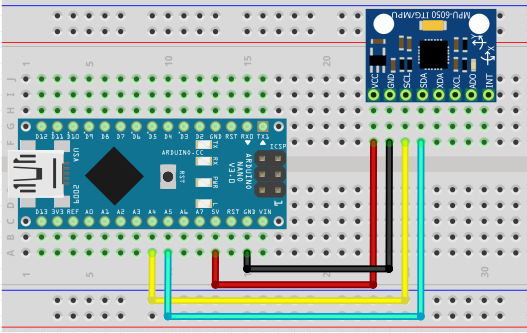
\includegraphics[keepaspectratio=true,scale=0.5]{figuras/conexoes_mpu_arduino.PNG}
			\caption{ Esquemático de conexão do MPU6050 com Arduino Nano }
			Fonte: autoria própria. \footnotesize
			\label{conexoes}	
		\end{figure}
		
		A comunicação entre o sensor MPU6050 e o Arduino foi realizada através do protocolo I2C, onde os dados eram enviados de forma serial através de apenas um fio e os dados organizados como mostrado na Figura \ref{comunicacao}, onde é evidenciado quais são os dados transmitidos do MPU6050 para o Arduino e a velocidade do \textit{clock}, e Figura \ref{i2c}, que mostra com mais detalhe a relação dos dados com o \textit{clock} .
		
		\begin{figure}[h]
			\centering
			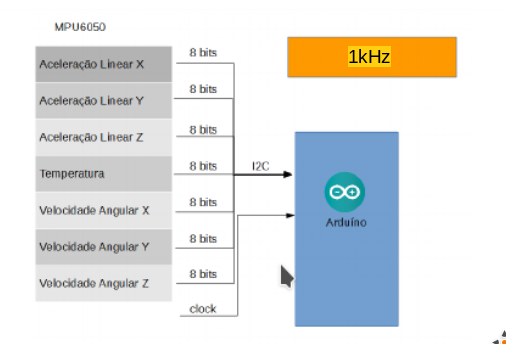
\includegraphics[keepaspectratio=true,scale=0.4]{figuras/comunicacao.PNG}
			\caption{ Transmissão de dados do MPU6050 para Arduino}
			Fonte: autoria própria. 
			\label{comunicacao}	
		\end{figure}
		
		\begin{figure}[h]
			\centering
			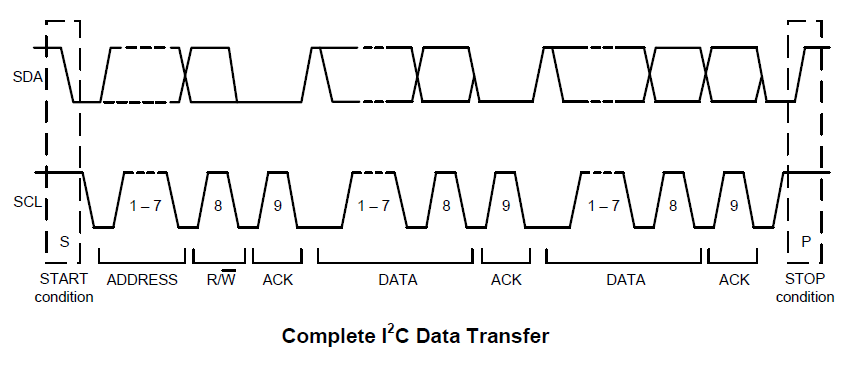
\includegraphics[keepaspectratio=true,scale=0.5]{figuras/i2c.PNG}
			\caption{Transferência de dados com o protocolo I2C. }
			Fonte: \cite{mpu6050}. 
			\label{i2c}	
		\end{figure}
	
		O Arduino Nano foi conectado ao computador por meio de um cabo USB 2.0, que além de ser responsável pela comunicação, também era por meio dele que era realizada a alimentação de energia com 5V de tensão. O protocolo de comunicação utilizado com um cabo USB também serial. Então os dados transmitidos do Arduino para o computador são enviados em série. 
		
		
\section {Projeto de Software}
		
		Para esse projeto foram necessários dois projetos de softwares, um para ficar salvo no Arduino e outro que será o software, em Python, responsável por fazer o tratamento dos dados adquiridos do sensor e salva-los para análises futuras.
		
		\subsection{Software para o Arduino}
			Os requisitos do software salvo no microcontrolador são:
			\begin{itemize}
				\item Inicializar o MPU6050;
				\item Receber os dados do MPU6050; 
				\item Enviar os dados para interface serial.
			\end{itemize}
		
		Para isso foi utilizada as bibliotecas \textit{Wire.h},\textit{I2Cdev.h} e \textit{MPU6050.h}, que são responsaveis por realizar a comunicação em I2C, enviar o comando de inicialização, a variável escolhida pelo usuário para definir os limites de leitura do acelerômetro e do giroscópio, e são estas bibliotecas que realizam a leitura dos registradores que tem o valor de cada sensor armazenado neles.  
		
		O fluxograma do software responsável pela leitura dos dados do MPU6050 e envio para a interface de comunicação serial é o mostrado na Figura \ref{fluxograma_arduino}. 
		
		\begin{figure}[h]
			\centering
			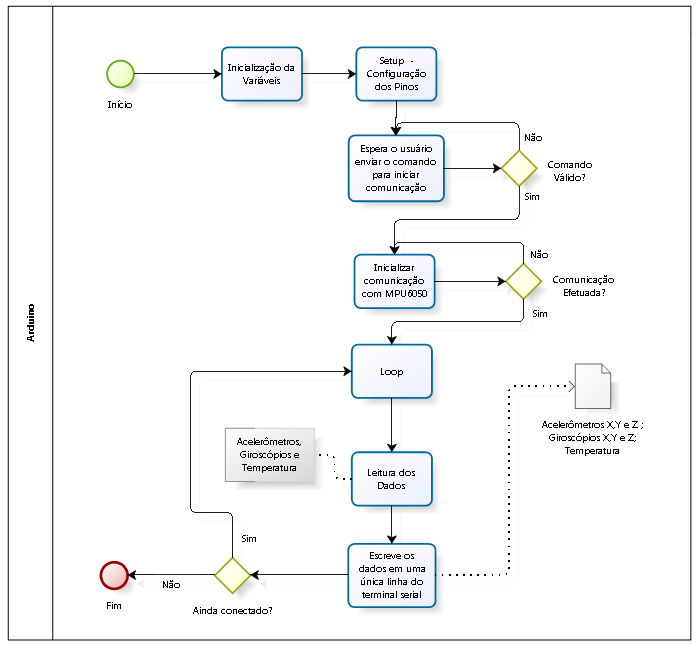
\includegraphics[keepaspectratio=true,scale=0.9]{figuras/diagrama_embarcado.PNG}
			\caption{Fluxograma do software de leitura dos dados. }
			Fonte: autoria própria. 
			\label{fluxograma_arduino}	
		\end{figure}
		
		Para realizar a transmissão dos dados do Arduino para o programa em Python, o programa salvo no Arduino imprime no terminal serial os dados obtidos do sensor. O programa é fechado sempre que uma nova leitura é realizada.
		 
\subsection{Software para Salvar os Dados}
		Esse segundo programa, foi feito para realizar a leitura dos dados transmitidos pelo Arduino, e salvar-los em um arquivo de texto, para futuras análises. Esse software ainda da a possibilidade do usuário salvar os dados sem nenhum tratamento ou os valores com medidas físicas aproximadas das medições realizadas. 
		
		O software foi escrito em Python 3 e compilado com o Jupyter Notebook e com a IDE Spyder, os dois compiladores são do pacote Anaconda. 
		
		O programa inicia mostrando a lista de dispositivos USB conectados ao computador, se não houver nenhum dispositivo conectado aparece a mensagem "Conecte o Arduino", se houver, a mesagem que aparece pede para digitar o número correspondente ao dispositivo que o usuário pretende verificar os dados. 
		
		Após a escolha do Arduino, o usuário deve escolher entre as 4 possibilidades de escala dos dados obtidos. E em seguida pressionar "enter" para iniciar a leitura e "Ctrl+C"\footnote{No Jupyter Notebook o "Ctrl+C" não funcionou, precisando assim pressionar o ícone de \textit{"stop"} disponível na tela.} para pausar e salvar os valores. O programa então imprime na tela os valores dos sensores que estão sendo lidos e ao fim do código, quando o usuário pressionar "Ctrl+C", os valores são salvos em dois arquivos nomeados com a data de quando foi finalizada a leitura, como mostrado na Figura \ref{fluxograma_python} .
		
		Para definir melhor os requisitos do software, foi feita a seguinte história de usuário descrita na Tabela \ref{User_story}
		
			\begin{table}[h] \footnotesize
			\centering
			\caption{História de Usuário}
			\label{User_story}
			
			\begin{tabular}{ccl}
				\toprule
				\textbf{Usuário} & \textbf{O que quer fazer?} & \textbf{Resposta do Sistema} \\
				\midrule
				Pesquisador & Inicializar o sistema &  Abre o prompt de comando \\
				 & & Mostra a lista de dispositivos conectados \\
				Pesquisador & Selecionar o sensor & Estabelecer a conexão com sensor \\
				& & Mostra a lista de intervalo de leitura\\
				Pesquisador & Selecionar o intervalo & Mensagem de qual intervalo foi selecionado\\
				& & Aguarda comando para iniciar a coleta\\
				Pesquisador & Iniciar coleta & Inicia a coleta\\
				& &  Aguarda comando para pausar coleta\\
				Pesquisador & Pausar coleta e salvar Dados & Para a coleta\\
				& & Fecha a conexão\\
				& & Salva os dados coletados\\
				& & Mensagem com nome dos arquivos\\  
 				
				\bottomrule
				 & & Fonte: autoria própria
			\end{tabular}
		\end{table}
		
		
 
		\begin{figure}[h]
			\centering
			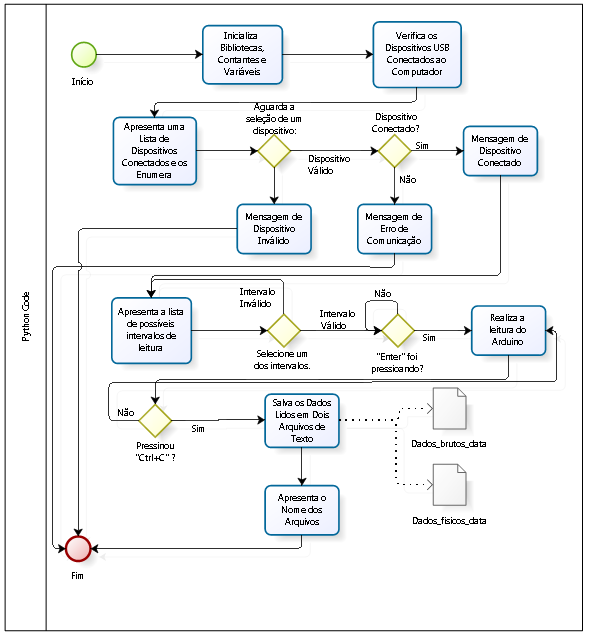
\includegraphics[keepaspectratio=true,scale=1]{figuras/diagrama_python.png}
			\caption{Fluxograma do software que salva os dados lidos. }
			Fonte: autoria própria. 
			\label{fluxograma_python}	
		\end{figure}
		
\section {Validação}

	Para testar o funcionamento dos acelerômetros do IMU, foi feito um teste simples. Pois o sempre que o sensor estiver "parado", ele estará sobre efeito da força peso e consequentemente da aceleração da gravidade de aproximadamente 9,8 m/$ s^2 $. Então para verificar, foi necessário testar o sensor com um eixo de cada vez alinhado com a normal, como na seguinte Figura .
	
	Após realizar as leitura, os dados foram plotados em um gráfico simples, onde o eixo horizontal representa o tempo e o vertical a aceleração medida. Foram colocados os gráficos dos 3 eixos na mesma imagem. 
	
	Para verificar o funcionamento do MPU6050  e se as leituras são confiáveis ou não serão necessários muitos outros teste além dos realizados até o momento.
	
	\textit{ESTUDO DE CASO}
	
	
	
\chapter{Resultados e Discussão}
	
	\textit{RESULTADOS:Fotos microcontrolador; fotos imu; gráficos; programas;ARQUIVOS SALVOS.}
		
	\textit{DISCUSSÃO: tempo para desenvolver interface gráfica. responder o porque dos erros, e o porque das escolhas. Ruído devido ao movimento do próprio corpo humano. 	
	}
\chapter{Conclusão}

	\textit{Feito protótipo, software para pesquisador, próximas etapas: case miniaturizado, comunicação sem fio.}